\documentclass[a4paper]{article}
\usepackage[warn]{mathtext}
\usepackage[utf8]{inputenc}
\usepackage[T2A]{fontenc}
\usepackage[english,russian]{babel}
\usepackage{indentfirst}
\usepackage{misccorr}
\usepackage{subcaption}
\captionsetup{compatibility=false}
\usepackage{geometry}
\geometry{verbose,a4paper,tmargin=2cm,bmargin=2cm,lmargin=1.5cm,rmargin=1.5cm}
\usepackage{graphicx}
\usepackage{wrapfig}
\usepackage{amsmath}
\usepackage{fancyhdr}
\usepackage{floatflt}
\usepackage{float}
\usepackage{amssymb}
\usepackage{color}
\usepackage{lscape}
\usepackage{hvfloat}
\usepackage{amsfonts}
\usepackage{euscript}
\usepackage{newunicodechar}
\usepackage{booktabs}
\usepackage{listings}
\usepackage{xcolor}

\definecolor{codegreen}{rgb}{0,0.6,0}
\definecolor{codegray}{rgb}{0.5,0.5,0.5}
\definecolor{codepurple}{rgb}{0.58,0,0.82}
\definecolor{backcolour}{rgb}{0.95,0.95,0.92}

\lstdefinestyle{mystyle}{
    backgroundcolor=\color{backcolour},   
    commentstyle=\color{codegreen},
    keywordstyle=\color{magenta},
    numberstyle=\tiny\color{codegray},
    stringstyle=\color{codepurple},
    basicstyle=\ttfamily\footnotesize,
    breakatwhitespace=false,         
    breaklines=true,                 
    captionpos=b,                    
    keepspaces=true,                 
    numbers=left,                    
    numbersep=5pt,                  
    showspaces=false,                
    showstringspaces=false,
    showtabs=false,                  
    tabsize=2
}

\lstset{style=mystyle}


\begin{document}
\newcommand{\apple}{\char"F8FF}

\begin{titlepage}
	\centering
	\vspace{5cm}
    {\scshape\LARGE Московский физико-технический институт\par}


	\vspace{3cm}
	{\scshape\Large Лабораторная работа по параллельному программированию \par}
	\vspace{1cm}
	{\huge\bfseries  Численное решение уравнения переноса с использованием технологии MPI \par}
	\vspace{1cm}
	\vfill
\begin{flushright}
	{\large выполнила студентка Б01-907 группы}\par
	\vspace{0.3cm}
	{\LARGE Юлия Прохорова }
\end{flushright}
	
	\vfill
Долгопрудный, 2022
% Bottom of the page
\end{titlepage}

\tableofcontents

\newpage

\section{Задание к выполнению}
\begin{enumerate}
    \item Разработать с помощью технологии MPI параллельную программу,
     которая численно решает уравнение переноса по разностной схеме в соответствии с индивидуальным вариантом
\end{enumerate}

\section{Теория}

\subsection{Эффективность и ускорение параллельных программ}

Основная цель параллельных вычислений - ускорение решения вычислительных задач. \par
Основные особенности:
\begin{enumerate}
    \item осуществляется управление работой множества процессов;
    \item организуется обмен данными между процессами;
    \item утрачивается детерминизм поведения в следствие асинхронности доступа к данным;
    \item преобладают нелокальные и динамические ошибки;
    \item появляется возможность тупиковых ситуаций;
    \item возникают проблемы масштабируемости программы и балансировки загрузки вычислительных узлов.
\end{enumerate}

Время выполнения параллельной версии алгоритма - $T_p = \alpha T_1 + \frac{(1-\alpha)T_1}{p}$,
 где $T_1$ - время выполнения последовательной программы. \par
Ускорение - $S= \frac{T_1}{T_p}$ \par
Эффективность - $E=\frac{S}{p}$ \par
Теоретическая оценка максимального ускорения (закон Амдаля) - $S=\frac{T_1}{T_p}=\frac{T_1}{\alpha T_1 + \frac{(1-\alpha)T_1}{p}} \leq \frac{1}{\alpha}$

\subsection{Основные понятия технологии MPI}

MPI - программный интерфейс для передачи сообщений между процессами. \par
На каждом вычислительном узле запускается копия параллельной программы. Каждая копия получает свой ранг - 
уникальный индификатор, используемый для адресации сообщений. Коммуникатор - способ группировки процессов (по умолчанию MPI\_COMM\_WORLD). \par
Cтруктура программы и основные понятия MPI
\begin{enumerate}
    \item Подключение библиотеки MPI.
    \item Инициализация среды MPI - MPI\_Init(*argc, *argv).
    \item Работа программы, обмен сообщениями.
    \item Остановка среды MPI - MPI\_Finalize().
\end{enumerate}

Узнать ранг процесса - MPI\_Comm\_rank(MPI\_COMM\_WORLD, *rank) \par
Общее число процессов  - MPI\_Comm\_size(MPI\_COMM\_WORLD, *size) \\

MPI\_Send(buffer, count, type, dst, tag, comm) - блокирующая отправка \par
MPI\_Isend(buffer, count, type, dst, tag, comm, request) - неблокирующая отправка \par
MPI\_Recv(buffer, count, type, src, tag, comm, status) - блокирующий прием \par 
MPI\_Irecv(buffer, count, type, src, tag, comm, request) - неблокирующий прием. \\

Параметры всех этих функций очень похожи: \\
buffer - указатель на начало области памяти, откуда передают/куда принимают данные \\
count - число элементов в буфере \\
type - тип элеметна в буфере \\
dst/src - ранг принимающего/передающего процесса \\
tag - метка сообщения \\
comm - коммуникатор, в рамках которого ведется обмен \\
status - указатель на структуру, в которой информация о статусе доставки \\
request - указатель на структуру, в которой будет информация о статусе доставки сообщения


\section{Условие}

Поиск численного решения для уравнения переноса:
$$\frac{\partial u(t,x)}{\partial t} +a\cdot\frac{\partial u(t,x)}{\partial x} = f(t,x), \; 0\leq t\leq T, \; 0\leq x \leq X$$
$$u(0, x) = \phi(x), 0\leq x \leq X$$
$$u(t, 0) = \psi(x), 0\leq t \leq T$$
\section{Код программы}

{\small
\begin{verbatim}

	#include<stdio.h>
	#include<iostream>
	#include<mpi.h>
	#include <iomanip>
	#include<vector>
	
	using namespace std;
	
	#define SIZE_X 10
	#define SIZE_T 10
	
	
	int M = SIZE_X; // по х
	int K = SIZE_T; // по t
	
	//будем рассматривать линейный случай
	double tau = 0.01;
	double h = 0.01;
	
	double phi(double x) {
		return x;
	}
	
	double ksi(double t) {
		return t;
	}
	
	double f(double t, double x) {
		return 0;
	}
	
	//Решение крестом
	double solve(double left, double right, double bottom, double f) {
		return bottom + 2 * tau * (f + (left - right) / (2 * h));
	}
	
	//Решение явной центральной трехточечной схемой на нижней границе
	double solve_bottom(double left, double right, double f) {
		return 0.5 * (left + right) + tau * (f + (left - right) / (2 * h));
	}
	
	//Решение уголком на правой границе
	double solve_right(double left, double central, double f) {
		return central + tau * (f + (left - central) / h);
	}
	
	//отправкка данных
	void data_send(double** data, MPI_Status& status, int ProcNum, int ProcRank, int N_PerProcess, int k);
	
	//прием данных
	pair<double, double> data_recive(double** data, 
									MPI_Status& status, int ProcNum, int ProcRank, int N_PerProcess, int k);
	
	//выделение памяти под матрицу
	template <typename T>
	T** new_matrix(int height, int width) {
		T** matrix = new T * [height];
		for (int i = 0; i < height; ++i) {
			matrix[i] = new T[width];
		}
		return matrix;
	}
	
	//удаление матрицы
	template <typename T>
	void delete_matrix(T** matrix, int height) {
		for (int i = 0; i < height; ++i) {
			delete[] matrix[i];
		}
		delete[] matrix;
	}
	
	int main(int argc, char* argv[]) {
	
		int ProcNum;
		int ProcRank;
	
		MPI_Status status;
	
		double time_d = 0;
		double time_end = 0;
		
		int N_PerProcess, N_Add;
		int FirstX;
	
		double time_start = MPI_Wtime();
		// Инициализируем среду MPI
		MPI_Init(&argc, &argv); 
		// Опереляем ранг текущего процесса
		MPI_Comm_rank(MPI_COMM_WORLD, &ProcRank);
		// Определяем общее количество процессов
		MPI_Comm_size(MPI_COMM_WORLD, &ProcNum);
	
		if (ProcRank == 0) {
			cout << "From process " << ProcRank << ": calculations begin" << endl;
		}
	
		//определяем количество точек для каждого процесса
		N_PerProcess = M / ProcNum;
		N_Add = M % ProcNum;
	
		if (ProcRank < N_Add) {
			N_PerProcess++;
			//определяем номер элеманта, с которого начнутся вычисления этого процесса
			FirstX = N_PerProcess * ProcRank;
		}
		else {
			FirstX = N_Add + N_PerProcess * ProcRank;
		}
	
		double** data = new_matrix<double>(K, N_PerProcess);
	
		// Процесс вычисляет свою часть значений в 1ой строке
		for (int n = 0; n < N_PerProcess; ++n) data[0][n] = phi((n + FirstX) * h);
	
		// Обмен данными для полноценного заполнения первой строки
		data_send(data, status, ProcNum, ProcRank, N_PerProcess, 0);
	
		// Получение  значения 1ой строки
		pair<double, double> data_recv = data_recive(data, status, ProcNum, ProcRank, N_PerProcess, 0);
		
		// Заполнение середины 2ой строки (также по частям)
		for (int n = 1; n < N_PerProcess - 1; ++n) 
			data[1][n] = solve_bottom(data[0][n - 1], data[0][n + 1], f(tau, (FirstX + n) * h));
	
		// Определение первого значения (своей группы) в 2ой строке
		if (ProcRank == 0)
			data[1][0] = ksi(tau);
		else				
			data[1][0] = solve_bottom(data_recv.first, data[0][1], f(tau, FirstX * h));
	
		// Определение последнего значения (своей группы) 2ой строки
		if (ProcRank == ProcNum - 1)	
			data[1][N_PerProcess - 1] = 
			solve_right(data[0][N_PerProcess - 2], data[0][N_PerProcess - 1], f(tau, h * (FirstX + N_PerProcess - 1)));
		else
			data[1][N_PerProcess - 1] = 
			solve_bottom(data[0][N_PerProcess - 2], data_recv.second, f(tau, h * (FirstX + N_PerProcess - 1)));
	
		// Отступили от края - можно считать для всех остальных
		for (int k = 2; k < K; ++k) {
			
			// Пересылка данных
			data_send(data, status, ProcNum, ProcRank, N_PerProcess, k - 1);
	
			// Значения в середине
			for (int n = 1; n < N_PerProcess - 1; ++n) 
			data[k][n] = solve(data[k - 1][n - 1], data[k - 2][n], data[k - 1][n + 1], f(k * tau, (FirstX + n) * h));
	
			// Получение данных
			pair<double, double> data_recv = data_recive(data, status, ProcNum, ProcRank, N_PerProcess, k - 1);
	
			// Граничное условие слева
			if (ProcRank == 0) data[k][0] = ksi(k * tau);
			else data[k][0] = solve(data_recv.first, data[k - 2][0], data[k - 1][1], f(k * tau, FirstX));
	
			// Граничное условие справа 
			if (ProcRank == ProcNum - 1) data[k][N_PerProcess - 1] = solve_right(data[k - 1][N_PerProcess - 2], 
									data[k - 1][N_PerProcess - 1], f(k * tau, (FirstX + N_PerProcess - 1) * h));

			else data[k][N_PerProcess - 1] = solve(data[k - 1][N_PerProcess - 2], 
			data[k - 2][N_PerProcess - 1], data_recv.second, f(k * tau, (FirstX + N_PerProcess - 1) * h));
		}
	
		//Сбор посчитанных данных в процесс 0
		if (ProcRank != 0) {
			double* reviving_data = new double[N_PerProcess * K];
	
			// Подготовка массива для данных
			for (int y = 0; y < K; ++y)
				for (int x = 0; x < N_PerProcess; ++x) reviving_data[y * N_PerProcess + x] = data[y][x];
	
			// Отправление количество элеменнтов, обрабатываемых процессом
			MPI_Send(&N_PerProcess, sizeof(N_PerProcess), MPI_BYTE, 0, 1, MPI_COMM_WORLD);
			// Отправление номера элемента, с которого начинал
			MPI_Send(&FirstX, sizeof(FirstX), MPI_BYTE, 0, 1, MPI_COMM_WORLD);
			// Отправление данных
			MPI_Send(reviving_data, N_PerProcess * K * sizeof(double), MPI_BYTE, 0, 1, MPI_COMM_WORLD);
	
			cout << "From process " << ProcRank << ": data sended to process 0 succesfully " << endl;
	
			delete[] reviving_data;
		}
		else {
			double** finale_data = new_matrix<double>(K, M);
			for (int y = 0; y < K; ++y)
				for (int x = 0; x < N_PerProcess; ++x)
					finale_data[y][x] = data[y][x];
	
			// Принимаем данных
			for (int i = 1; i < ProcNum; ++i) {
	
				// Колличество обрабатываемых столбцов у процесса, который пересылает данные
				int rec_N_PerProcess;
				MPI_Recv(&rec_N_PerProcess, sizeof(rec_N_PerProcess), MPI_BYTE, i, 1, MPI_COMM_WORLD, &status);
	
				// Номер элемента, с которого начанался рассчет
				int proc_FirstX;
				MPI_Recv(&proc_FirstX, sizeof(proc_FirstX), MPI_BYTE, i, 1, MPI_COMM_WORLD, &status);
	
				// Значения
				double* reciving_data = new double[rec_N_PerProcess * K];
				MPI_Recv(reciving_data, rec_N_PerProcess * K * sizeof(double), MPI_BYTE, i, 1, MPI_COMM_WORLD, &status);
	
				cout << "From process " << ProcRank << ": data recived from process  " << i << " succesfully" << endl;
	
				for (int iy = 0; iy < K; ++iy)
					for (int ix = 0; ix < rec_N_PerProcess; ++ix)
						finale_data[iy][ix + proc_FirstX] = reciving_data[iy * rec_N_PerProcess + ix];
			}
	
			// Затраченное время
			time_end = MPI_Wtime();
			time_d = time_end - time_start;
	
			cout << "From process " << ProcRank << ": calculations completed. Time " << time_d << " seconds" << endl;
	
			cout << endl <<  "Final data: "  << endl << endl;
	
			cout << fixed;
			cout.precision(2);
	
			// Вывод рассчитанных данных
			for (int iy = 0; iy < K; ++iy) {
				for (int ix = 0; ix < M; ++ix) {
					cout << setw(10) << finale_data[iy][ix] << " ";
				}
				cout << endl;
			}
	
			delete_matrix<double>(finale_data, K);
		}
	
		delete_matrix<double>(data, K);
	
		MPI_Finalize();
	
		return 0;
	}
	
	//отправкка данных
	void data_send(double** data, MPI_Status& status, int ProcNum, int ProcRank, int N_PerProcess, int k) {
		
		double send_right, send_left;
	
		if (ProcRank == 0) {
			send_right = data[k][N_PerProcess - 1];
			MPI_Send(&send_right, sizeof(send_right), MPI_BYTE, 1, 1, MPI_COMM_WORLD);
		}
		else if (ProcRank == ProcNum - 1) {
			send_left = data[k][0];
			MPI_Send(&send_left, sizeof(send_left), MPI_BYTE, ProcRank - 1, 1, MPI_COMM_WORLD);
		}
		else {
			send_right = data[k][N_PerProcess - 1];
			MPI_Send(&send_right, sizeof(send_right), MPI_BYTE, ProcRank + 1, 1, MPI_COMM_WORLD);
			send_left = data[k][0];
			MPI_Send(&send_left, sizeof(send_left), MPI_BYTE, ProcRank - 1, 1, MPI_COMM_WORLD);
		}
	}
	
	//прием данных
	pair<double, double> data_recive(double** data, 
	MPI_Status& status, int ProcNum, int ProcRank, int N_PerProcess, int k) {
		
		double recv_right, recv_left;
	
		if (ProcRank == 0) {
			MPI_Recv(&recv_right, sizeof(recv_right), MPI_BYTE, 1, 1, MPI_COMM_WORLD, &status);
			recv_left = 0;
		}
		else if (ProcRank == ProcNum - 1) {
			MPI_Recv(&recv_left, sizeof(recv_left), MPI_BYTE, ProcRank - 1, 1, MPI_COMM_WORLD, &status);
			recv_right = 0;
		}
		else {
			MPI_Recv(&recv_right, sizeof(recv_right), MPI_BYTE, ProcRank + 1, 1, MPI_COMM_WORLD, &status);
			MPI_Recv(&recv_left, sizeof(recv_left), MPI_BYTE, ProcRank - 1, 1, MPI_COMM_WORLD, &status);
		}
	
		return pair<double, double>(recv_left, recv_right);
	}

\end{verbatim}
}

\section{Результат}
\begin{figure}[h]
	\center{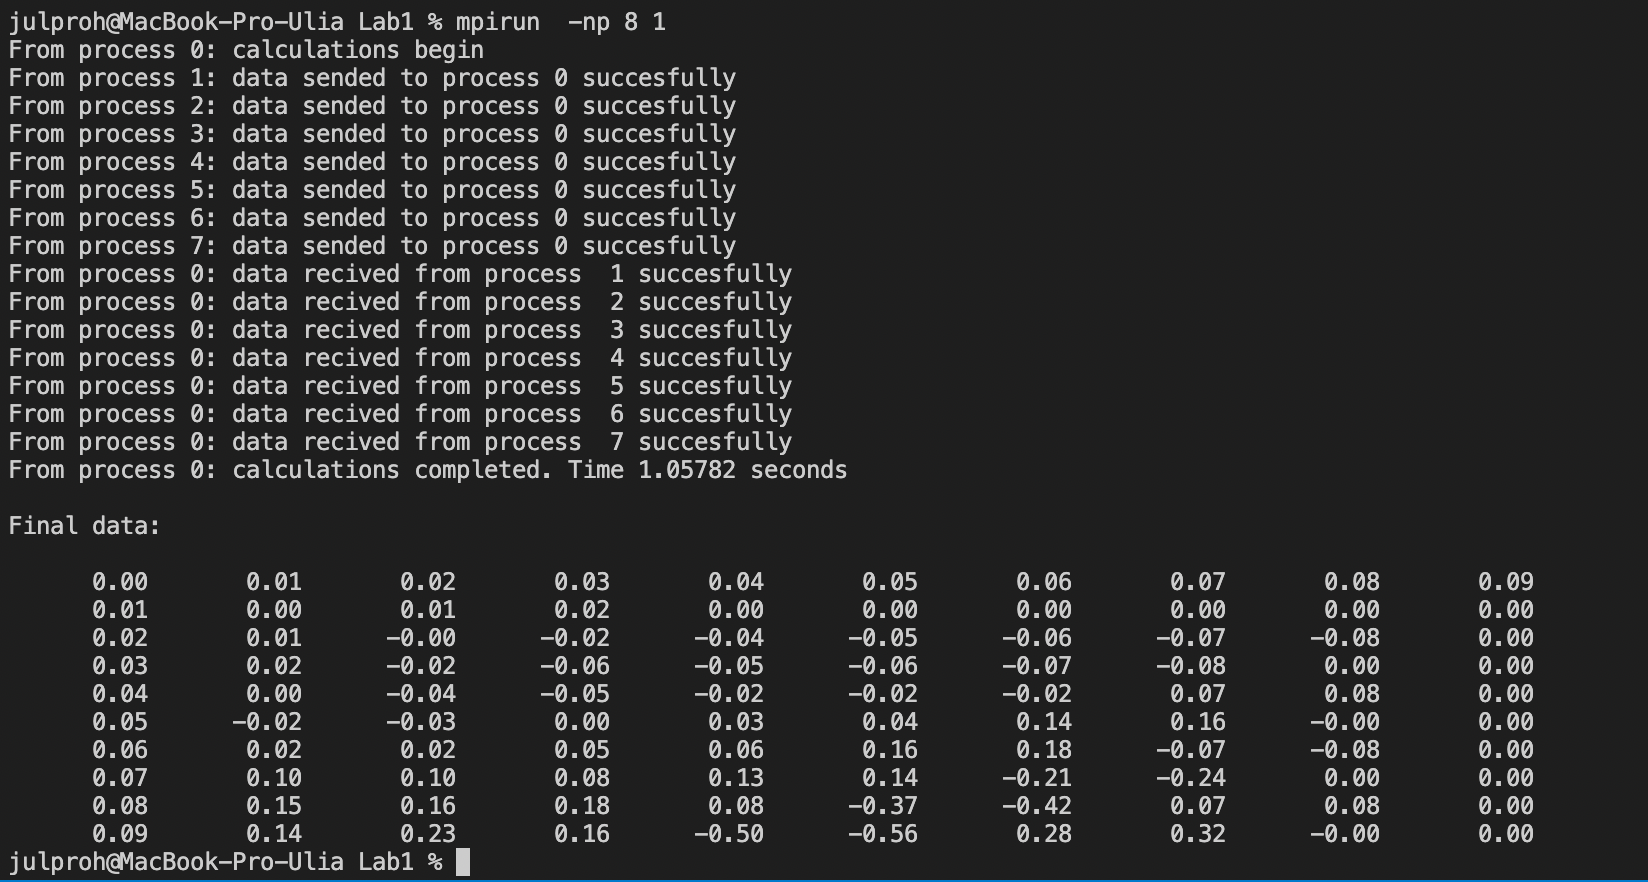
\includegraphics[width=1\linewidth]{output.png}}
	\caption{Полученный результат.}
	\end{figure}

\section{Контрольные вопросы}

\begin{enumerate}

\item Ускорение и эффективность параллельных алгоритмов. \par
 	Ускорение - $S= \frac{T_1}{T_p}$ \\
	Эффективность - $E=\frac{S}{p}$ 
\item Закон Амдаля. \par
$$S=\frac{T_1}{T_p}=\frac{T_1}{\alpha T_1 + \frac{(1-\alpha)T_1}{p}} \leq \frac{1}{\alpha}$$
\item Свойства канала передачи данных. Латентность. \par
Основными характеристиками быстродействия сети являются латентность и пропускная способность. 
\begin{enumerate}
	\item Пропускная способность сети определяется количеством информации, 
	передаваемой между узлами сети в единицу времени. Реальная пропускная способность снижается программным обеспечением за счет передачи служебной информации.
	\item Латентностью (задержкой) называется время, затрачиваемое программным обеспечением
	 и устройствами сети на подготовку к передаче информации по данному каналу.
	  Полная латентность складывается из программной и аппаратной составляющих.
\end{enumerate}

Различают следующие виды пропускной способности сети:
\begin{enumerate}
	\item Пропускная способность однонаправленных пересылок -  максимальная скорость, с которой процесс на одном узле может передает данные процессу на другом узле.

	\item Пропускная способность двунаправленных пересылок -  максимальная скорость, с которой два процесса могут одновременно обмениваться данными по сети.

\end{enumerate}


\item Виды обменов "точка-точка"
		\begin{enumerate}
			\item Синхронные:
				\begin{enumerate}
					\item MPI\_Send(buffer, count, type, dst, tag, comm) 
					\item MPI\_Recv(buffer, count, type, src, tag, comm, status) 
				\end{enumerate}
			\item Асинхронные:
				\begin{enumerate}
					\item MPI\_ISend(buffer, count, type, dst, tag, comm, request) 
					\item MPI\_IRecv(buffer, count, type, src, tag, comm, request) 
				\end{enumerate}
		\end{enumerate}
		Буфферизация данных - предполагает предварительное явное выделение блока, 
		который будет использоваться для группировки (буферизации) посылаемых данных. 
		Это гарантирует, что необходимое количество места для посылаемых данных является доступным.
\item Балансировка загрузки
\begin{enumerate}
	\item Статическая выполняется до начала выполнения распараллеленой программы. 
	Однако не всегда оказывает необходимый эффекта, так как вычислительный узел, на котором выполняется программа может быть занят другими вычислениями.

	\item Динамическая балансировка предусматривает перераспределение вычислительной
	 нагрузки на узлы во время выполнения программы.
\end{enumerate}

\item Геометрический параллелизм. \par
Геометрическим параллелизмом обладают многие физические задачи, которые описываются дифференциальными уравнениями в частных производных. Такие задачи обычно решаются конечно-разностными методами -
разбиение области решения задачи на подобласти и вычисления в каждой из подобластей поручить отдельному процессору. Отличие геометрического параллелизма от параллелизма по данным состоит в том, что в подобласти 
взаимосвязаны (требуется обмен данными между этими подзадачами).

\item Конвейнерный параллелизм. \par
Типичный пример конвейерного параллелизма представляет собой параллелизм систем обработки видеоинформации. В таких системах множество изображений должны проходить несколько этапов обработки.
Конвейерную декомпозицию задачи - каждый этап обработки выполняется на отдельном процессоре.
Конвейерная декомпозиция имеет весьма ограниченное применение, поскольку весьма редко удается организовать достаточно длинный конвейер и обеспечить равномерную загрузку всех процессоров.




\end{enumerate}

\end{document}